%%%%%%%%%%%%%%%%%%%%%%%%%%%%%%%%%%%%%%%%%%%%%%%%%%%%%%%%%%%%%%%%%%%%%%%%%%%%%%%%%%
\begin{frame}[fragile]\frametitle{}
\begin{center}
{\Large Chatbots in Healthcare}
\end{center}
\end{frame}

%%%%%%%%%%%%%%%%%%%%%%%%%%%%%%%%%%%%%%%%%%%%%%%%%%%%%%%%%%%
\begin{frame}[fragile]\frametitle{Health-care}
Top 8 Health-care Predictions for 2019

\begin{center}
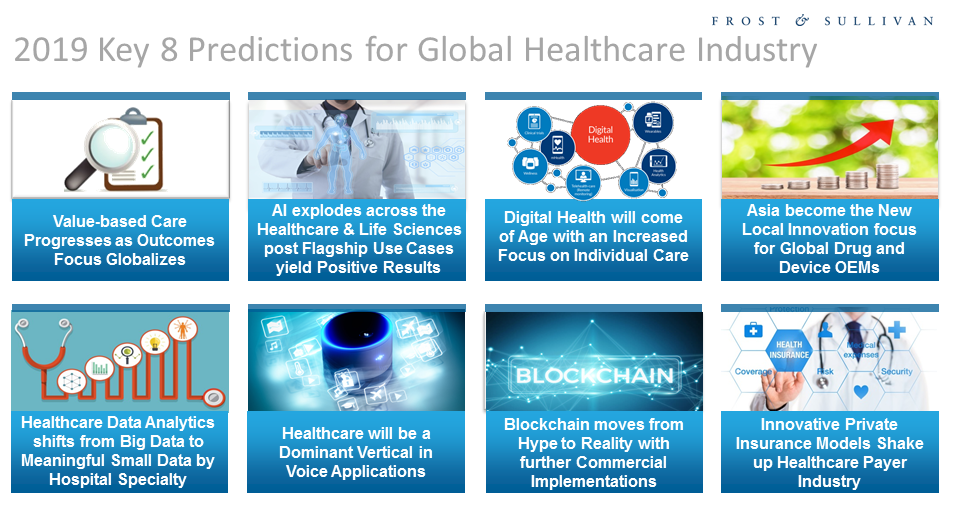
\includegraphics[width=0.9\linewidth]{healthcare1}
\end{center}

``HIPAA-compliant voice and chatbot applications for healthcare will gain prominence \ldots''

% {\tiny (Ref: Top 8 Healthcare Predictions for 2019 - FROST \& SULLIVAN/ Reenita Das)}
\end{frame}

%%%%%%%%%%%%%%%%%%%%%%%%%%%%%%%%%%%%%%%%%%%%%%%%%%%%%%%%%%%
\begin{frame}[fragile]\frametitle{Health-care}
How Artificial Intelligence is Changing the Health-care Industry

\begin{itemize}
\item Electronic Health Records
\item Medical Imaging Diagnostics
\item {\bf Virtual Health Assistance}
\begin{itemize}
\item Remind patients to take their medication at the appointed time
\item Provide medical advice when they have common ailments or complaints
\item  Suggest diet and eating habits for people with diet restrictions
\item  Remind when they are about to run out of medicines and order prescriptions
\item  Remind them of doctor appointments and manage bookings
\item  Allow virtual interaction with doctors
\end{itemize}
\item Robotic Assistance
\item Proactive Medical Care
\end{itemize}

Virtual Health Assistance aka chatbots have the potential to save clinics and hospitals thousands of dollars.

% {\tiny (Ref: How Artificial Intelligence is Changing the Healthcare Industry - Sumi menon)}
\end{frame}

%%%%%%%%%%%%%%%%%%%%%%%%%%%%%%%%%%%%%%%%%%%%%%%%%%%%%%%%%%%
\begin{frame}[fragile]\frametitle{Health-care Chatbot}

\begin{itemize}
\item  Potential to revolutionize the patient experience
\item Comes with its own costs and challenges.
\item So the real question for clinics, hospitals and other private practices looking to improve the patient experience with AI chatbots is this: Is it worth it?
\item Will chatbots really make a difference for your staff and patients?
\end{itemize}


% {\tiny (Ref: Can Healthcare Chatbots Improve the Patient Experience? - Intakeq)}
\end{frame}

%%%%%%%%%%%%%%%%%%%%%%%%%%%%%%%%%%%%%%%%%%%%%%%%%%%%%%%%%%%
\begin{frame}[fragile]\frametitle{What are Health-care Chatbots?}

\begin{itemize}
\item Use Artificial Intelligence to automatically gather information from the Internet (or any information database) to predict, analyze and answer questions.
\item  Help doctors look up medication information, order supplies, write prescriptions and other practitioner-specific administrative tasks. 
\item Simply be used for advice.
\end{itemize}


% {\tiny (Ref: Can Healthcare Chatbots Improve the Patient Experience? - Intakeq)}
\end{frame}

%%%%%%%%%%%%%%%%%%%%%%%%%%%%%%%%%%%%%%%%%%%%%%%%%%%%%%%%%%%
\begin{frame}[fragile]\frametitle{Health-care Chatbots Examples}

\begin{columns}
\begin{column}[T]{0.5\linewidth}
\begin{itemize}
\item The first one: Eliza, for example, is a rudimentary chatbot that was originally developed to simulate a psychotherapist. AIML like.
\item HealthTap allows patients to learn more about their health by asking questions, check symptoms or conditions, and find relevant specialists if they need it.
\item Florence can remind patients to take their medication, help them stay motivated to stick to their schedules, and provide other relevant medical information.
\end{itemize}
\end{column}
\begin{column}[T]{0.5\linewidth}

\begin{center}
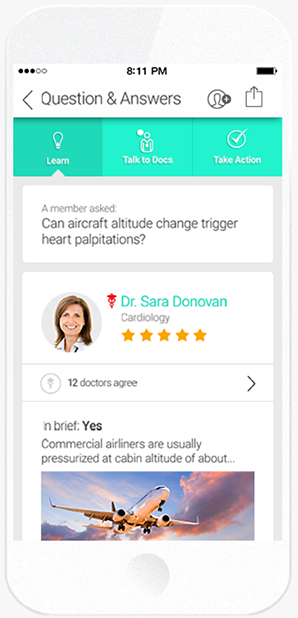
\includegraphics[width=0.25\linewidth]{hchat1}

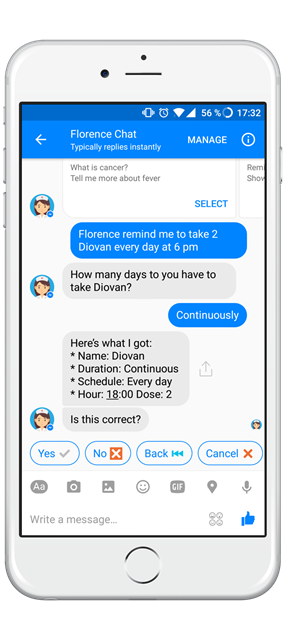
\includegraphics[width=0.25\linewidth]{hchat2}
\end{center}

\end{column}

\end{columns}

% {\tiny (Ref: Can Healthcare Chatbots Improve the Patient Experience? - Intakeq)}
\end{frame}

%%%%%%%%%%%%%%%%%%%%%%%%%%%%%%%%%%%%%%%%%%%%%%%%%%%%%%%%%%%
\begin{frame}[fragile]\frametitle{Benefits of Chatbots?}

\begin{itemize}
\item Cost savings: According to Juniper Research, chatbots could save organizations up to \$8 billion annually by 2022, a figure that was predicted to be at \$20 million just a year ago. Using bots can expect average time savings of just over four minutes per inquiry, equating to average cost savings in the range of \$0.50-\$0.70 per interaction.
\item Can improve at-home care.  ``Virtual nurses'' (like Florence) could help patients take their medications and connect with their primary care physicians.
\item Chatbots are more secure than a search engine. Are built with security protocols and requirements, making them a great HIPAA-compliant option for both patients and healthcare providers.
\end{itemize}


% {\tiny (Ref: Can Healthcare Chatbots Improve the Patient Experience? - Intakeq)}
\end{frame}

%%%%%%%%%%%%%%%%%%%%%%%%%%%%%%%%%%%%%%%%%%%%%%%%%%%%%%%%%%%
\begin{frame}[fragile]\frametitle{Build or Buy?}

\begin{itemize}
\item Hire a developer to build your own chatbot. The average app developer chargers \$6,453 for a single project.
\item Use a bot-as-a-service to build a custom chatbot, like Avaamo.
\item Use a pre-made chatbot (like HealthTap or Florence, etc.)
\end{itemize}


% {\tiny (Ref: Can Healthcare Chatbots Improve the Patient Experience? - Intakeq)}
\end{frame}